\chapter{Khoảng nhìn rõ và sự điều tiết của mắt}
\section{Lý thuyết trọng tâm}

\subsection{Sự điều tiết của mắt. Điểm cực viễn. Điểm cực cận}
\subsubsection{Sự điều tiết}
	Sự điều tiết của mắt là hoạt động của mắt làm thay đổi tiêu cự để cho ảnh của vật ở cách mắt những khoảng khác nhau vẫn được tạo ra trên màng lưới. 
	
	Mắt có thể điều tiết được là do các cơ vòng của mắt. Khi bóp lạị, các cơ này làm cho thể thủy tinh phồng lên, giảm bán kính cong, do đó tiêu cự của mắt giảm và ngược lại.
	
	Khi mắt ở trạng thái không điều tiết, tiêu cự của thấu kính mắt lớn nhất. Còn khi các cơ mắt bóp tối đa, mắt ở trạng thái điều tiết tối đa, khiến ta mỏi mắt nhất, thể thủy tinh phồng lên nhiều nhất, làm cho tiêu cự của thấu kính mắt lúc này nhỏ nhất.
	
\subsubsection{Điểm cực viễn. Điểm cực cận}
\begin{center}
	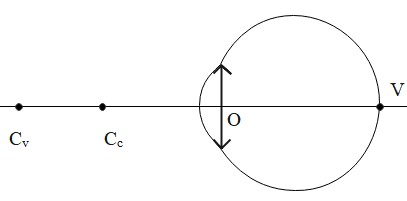
\includegraphics[scale=0.8]{../figs/VN11-PH-40-L-028-2-h34.jpg}
\end{center}

Khi mắt không điều tiết, võng mạc thu được ảnh của một vật đặt tại vị trí gọi là \textit{điểm cực viễn} $\text{C}_\text{v}$ của mắt. $\text{C}_\text{v}$ là điểm xa nhất mà mắt có thể nhìn thấy rõ. Đối với mắt bình thường, điểm cực viễn ở rất xa. 
	
Khi mắt điều tiết tối đa, võng mạc thu được ảnh của một vật đặt tại vị trí  gọi là \textit{điểm cực cận} $\text{C}_\text{c}$ của mắt. $\text{C}_\text{v}$ là điểm gần nhất mà mắt còn nhìn rõ. 

Mắt ta chỉ nhìn thấy rõ vật khi vật nằm trong khoảng từ cực viễn đến cực cận của mắt. Ta gọi đó là \textit{khoảng nhìn rõ} của mắt. Các khoảng $\text{O}\text{C}_\text{v}$, $\text{OC}_\text{c}$ lần lượt được gọi là \textit{khoảng cực viễn} và  \textit{khoảng cực cận }của mắt.

\subsection{Năng suất phân li của mắt}
Xét một vật có độ cao là AB, \textit{góc trông vật} là góc tạo bởi hai tia sáng xuất phát từ hai điểm A và B tới mắt.
\begin{center}
	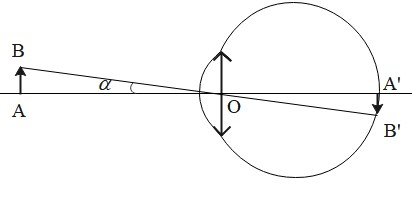
\includegraphics[scale=0.8]{../figs/VN11-PH-40-L-028-2-h35.jpg}
\end{center}

Góc trông nhỏ nhất khi nhìn vật AB mà mắt còn có thể phân biệt được hai điểm A và B, được gọi năng suất phân li, kí hiệu là $\varepsilon$.

Muốn mắt phân biệt được hai điểm A và B thì $\alpha$ lớn hơn hoặc bằng $\varepsilon$.

Năng suất phân li phụ thuộc vào mắt từng người, đối với mắt bình thường thì: 
\begin{equation}
\varepsilon=\alpha_{\text{min}}\approx 1'\approx 3\cdot 10^{-4}\ \text{rad}
\end{equation}



\section{Bài tập }
\begin{dang}{Tiêu cự và độ tụ của thể thủy tinh}
\end{dang}
\textbf{Phương pháp giải}

Khoảng cách từ thủy tinh thể O đến võng mạc V không đổi:
$$d'=\text{OC}_\text{V}= \textrm{hằng số}.$$

Gọi khoảng cách từ vật đến mắt là $d$, công thức xác định vị trí ảnh:
$$\dfrac{1}{f}=\dfrac{1}{d}+\dfrac{1}{d'}=\dfrac{1}{d}+\dfrac{1}{\text{OV}},$$ 
trong đó $f$ là tiêu cự của thủy tinh thể.

\begin{itemize}
	\item \textbf{Khi mắt nhìn vật ở cực cận} $\text{C}_\text{c}$: $d=\text{OC}_\text{c}$.
	
	Tiêu cự của thủy tinh thể lúc này cực tiểu:
	$$\dfrac{1}{f_\text{min}}=\dfrac{1}{\text{OV}}+\dfrac{1}{\text{OC}_\text{c}}.$$
	
	\item \textbf{Khi mắt nhìn vật ở cực viễn} $\text{C}_\text{v}$: $d=\text{OC}_\text{v}$.
	
	Tiêu cự của thủy tinh thể lúc này cực đại:
	$$\dfrac{1}{f_\text{max}}=\dfrac{1}{\text{OV}}+\dfrac{1}{\text{OC}_\text{v}}.$$
	
	\item \textbf{Khi điểm cực viễn ở xa vô cực} $(d=\infty)$:
	
	Độ biến thiên độ tụ của thủy tinh thể:
	$$\Delta D= D_{\text{max}}-D_{\text{min}}=\dfrac{1}{f_\text{min}}-\dfrac{1}{f_\text{max}}=\dfrac{1}{\text{OC}_\text{c}}-\dfrac{1}{\text{OC}_\text{v}}.$$
\end{itemize}
\vspace{1em}
\viduii{3}{
Một người có mắt bình thường, điểm cực viễn ở vô cực và điểm cực cận cách mắt 25 cm. Hiệu số giữa độ tụ cực đại và độ tụ cực tiểu của thủy tinh thể của mắt là 
\begin{mcq}(4)
	\item 2 dp.
	\item 4 dp.
	\item 6 dp.
	\item 8 dp.
\end{mcq}}
{\begin{center}
	\textbf{Hướng dẫn giải:}
\end{center}

 Theo đề bài: $\text{OC}_\text{c}=25\ \text{cm}, \ \text{OC}_\text{c}=\infty$.
	
	Ảnh thu được nằm trên màng lưới: $d'=\text{OV}$.
	
	Công thức thấu kính mắt: $D=\dfrac{1}{f}=\dfrac{1}{d}+\dfrac{1}{d'}=\dfrac{1}{d}+\dfrac{1}{\text{OV}}$.
	
	Khi mắt nhìn vật ở điểm cực cận: $d=\text{OC}_\text{c}$.
	
		$D_\text{max}=\dfrac{1}{f_\text{min}}=\dfrac{1}{\text{OV}}+\dfrac{1}{\text{OC}_\text{c}}=\dfrac{1}{\text{OV}}+\dfrac{1}{\text{0,25}}$.
		
		Khi mắt nhìn vật ở điểm cực viễn: $d=\text{OC}_\text{v}=\infty$.
		
			$D_\text{min}=\dfrac{1}{f_\text{max}}=\dfrac{1}{\text{OV}}+\dfrac{1}{\text{OC}_\text{v}}=\dfrac{1}{\text{OV}}+\dfrac{1}{\infty}=\dfrac{1}{\text{OV}}$.
			
		Hiệu số giữa độ tụ cực đại và độ tụ cực tiểu của thủy tinh thể của mắt là:
		
		 $\Delta D= D_{\text{max}}-D_{\text{min}}=\dfrac{1}{\text{0,25}}=4\ \text{dp}$.
		 
\textbf{	Đáp án: B.}
}

\viduii{3}{
Khoảng cách từ thuỷ tinh thể đến võng mạc bằng 15 mm. Tiêu cự của mắt biến đổi trong khoảng từ 14 mm đến $f_\text{max}$. Biết mắt người này bình thường, không bị tật. Tìm khoảng nhìn rõ của mắt người và độ biến thiên độ tụ của mắt khi chuyển trạng thái không điều tiết sang điều tiết tối đa
\begin{mcq}
	\item Khoảng nhìn rõ từ 14 cm đến vô cùng, độ biến thiên độ tụ $\Delta D\approx \text{2,67}\ \text{dp}$.
	\item Khoảng nhìn rõ từ 14 cm đến vô cùng, độ biến thiên độ tụ $\Delta D\approx \text{3,67}\ \text{dp}$.
	\item Khoảng nhìn rõ từ 21 cm đến vô cùng, độ biến thiên độ tụ $\Delta D\approx \text{4,67}\ \text{dp}$.
	\item Khoảng nhìn rõ từ 21 cm đến vô cùng, độ biến thiên độ tụ $\Delta D\approx \text{5,67}\ \text{dp}$.
\end{mcq}}
{\begin{center}
	\textbf{Hướng dẫn giải:}
\end{center}

{ Khoảng cách từ thể thủy tinh đến võng mạc: $d'=\text{OV}= 15\ \text{mm}=15\cdot 10^{-3}\ \text{m}$.
	
	Mắt bình thường, khi nhìn vật ở cực viễn thì $d=\infty$, tiêu cự lúc này đạt cực đại $f_\text{max}$.
	
	$D_\text{min}=\dfrac{1}{f_\text{max}}=\dfrac{1}{\text{OV}}+\dfrac{1}{\text{OC}_\text{v}}=\dfrac{1}{\text{OV}}+\dfrac{1}{\infty}=\dfrac{1}{\text{OV}}=\dfrac{200}{3}\ \text{dp}$.
	
	Khi mắt nhìn vật ở cực cận thì $d=\text{OC}_\text{c}$, tiêu cự lúc này đạt cực tiểu $f_\text{min}=14\ \text{mm}$.
	
	$D_\text{max}=\dfrac{1}{f_\text{min}}=\dfrac{500}{7}\ \text{dp}$.
	
	Ta có: $\dfrac{1}{f_\text{min}}=\dfrac{1}{\text{OV}}+\dfrac{1}{\text{OC}_\text{c}}\Rightarrow \text{OC}_\text{c}=210\ \text{mm}=21\ \text{cm}$.
	
	Phạm vi nhìn rõ của mắt người này từ 21 cm đến vô cùng.
	
	Độ biến thiên độ tụ của mắt khi chuyển trạng thái không điều tiết sang điều tiết tối đa là $\Delta D=D_\text{max}-D_\text{min}\approx \text{4,67}\ \text{dp}$.
	
	
	
	
	
	
\textbf{	Đáp án: C.}
}
}
\begin{dang}{Năng suất phân ly của mắt}
\end{dang}

\vidu{2}{
Một Người quan sát vật AB cao 4 cm cách mắt một đoạn $\text{OA}=\text{0,5}\ \text{m}$. 
\begin{center}
	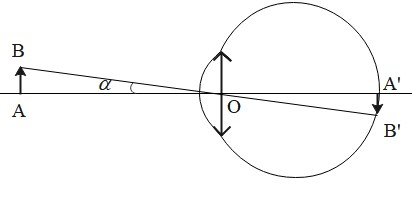
\includegraphics[scale=0.8]{../figs/VN11-PH-40-L-028-2-h35.jpg}
\end{center}
\begin{enumerate}
	\item Tính góc trông ảnh của vật qua mắt thường.
	\item Tìm độ cao nhỏ nhất $\text{A}_1\text{B}_1$ của vật mà mắt người còn có thể phân biệt được hai điểm $\text{A}_1,\text{B}_1$. Biết năng suất phân ly của mắt là $3\cdot 10^{-4}\ \text{rad}$ và vật $\text{A}_1\text{B}_1$  vẫn cách mắt một đoạn như trên. 
	
\end{enumerate}	
}
{
\begin{center}
	\textbf{Hướng dẫn giải:}
\end{center}

{\begin{enumerate}
	\item Dựa vào hình vẽ: $\tan \alpha = \dfrac{\text{AB}}{\text{OA}}=\text{0,08}\ \text{m}\Rightarrow \alpha =\text{79,8}\cdot 10^{-3}\ \text{rad}$.
		
	\item Gọi $\text{A}_1\text{B}_1$ là độ cao nhỏ nhất của vật.
	
	Dựa vào công thức: $\tan \alpha_{\text{min}}=\dfrac{\text{A}_1\text{B}_1}{\text{OA}_1}\Rightarrow \text{A}_1\text{B}_1=\text{OA}_1\cdot \tan \alpha_{\text{min}}=\text{1,5}\cdot 10^{-4}\ \text{m}=\text{0,15}\ \text{mm}$.

	\end{enumerate}

}
}